\chapter{Servlets}
Servletler html sayfaları ile java programları arasında bir nevi arayüz olarak tanımlanabilir. Kendileri de birer java programı olan bu kod parçalarının ana amacı MVC (model view controller) yaklaşımı
doğrultusunda iş (business-model) ile web arayüzü arasındaki iletişimi kontrol etmektir. Aslında sadece kontrol değil bizzat kendileri de sayfa generate etmek içinde kullanılabilirler. 

\section{Örnek Bir Program: Ön Giriş}
Projemizin dosya düzeni Şekil \ref{fig:filetree} de görüldüğü gibidir. Ön alt yapıyı maven ile otomatik de oluşturabiliriz. Bunun için bilgisayarınıza maven` ı yükledikten sonra konsolda mvn archetype:generate yazın. Sizden bir iskelet yapı seçmenizi isteyecek webapp yazın, ikinci çıkan listeden en temel web applicasyonunu seçin (güncel olaraka ikinci liste numarası 38).
\begin{figure}[h]
\centering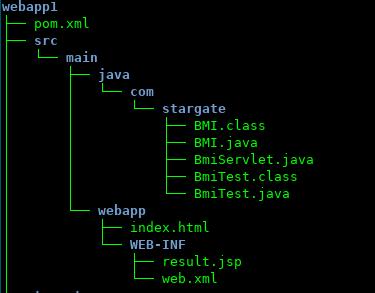
\includegraphics[scale=0.7]{/java/filetree}
\caption{\emph{"webapp1"} Projesinin Dosya Yapısı}
\label{fig:filetree}
\end{figure}
Projeyi derlemek ve hemen kullanıma koymak için maven aracını kullanmak bize büyük esneklik ve kolaylık sağlar. Altta olup bitenden çok kopmadan projenin kontrolü tamamen sizde olur. Özellikle ilk başta bir IDE kullanarak yapılan projeler genellikle ayrıntıya hakim olamama sorununa yol açabilir. 
Diğer bir yol ise javac ile derlemeleri yapıp manuel olarak classları yerlerine koymaktır ancak küçük projelerde bu yapılabilir olsa da biraz büyük projeler için ayrı bir iş yükü getireceğinden tavsiye edilmemektedir.

\subsection{Maven` a Kısa Bir Giriş}%
\label{sub:mavengiris}
C++ için \emph{make} neyse java için textbf{emph{Maven}} odur. Maven aslında  
sadece bir yapılandırma aracı (build tool) değil eklentili yapısı ile tüm projeyi
ve deployment` ı ayarlamaya ve şekillendirmeye yarayan bir araçtır.

Projenin derlenmesi için kaynak (src) klasörünün yanında \emph{pom.xml} adındaki
proje konfigurasyon dosyasının oluşturulması gerekir (Bkz. Şekil \ref{fig:filetree} ve Liste \ref{list:webpom}). Maven pom.xml dosyasında belirttiğimiz bağımlılıkları ve kütüphaneleri de otomatik olarak kurar.


\lstinputlisting[label={list:webpom},caption={Maven Yapılandırma Dosyası: pom.xml},language={XML},breaklines]{/home/cagatay/gitrepo/Ipa-ITBook/konular/java/projects/webProjects/webapp1/pom.xml}
Projeyi derlemek için pom dosyasının olduğu proje klasörü içerisinde \emph{mvn:compile} yazılır.
Projeyi server` a yüklemek için "\emph{mvn tomcat7:deploy}" veya daha önce yüklemiş ama güncellemek istiyorsak "\emph{mvn tomcat7:redploy}" yazmamız yeterlidir. Local serverımız da (http:localhost:8080/webapp1-1.0) altında projemizi inceleyebiliriz. Pom.xml içerisinde projenin yükleneceği adresi ve diğer ayarları yapabiliriz.

\subsection{Vücut Kütle Endeksi Programı, Örnek Projenin Ayakları}
Projemiz  MVC altyapısına uygun olarak biri karşılama diğeri sonuç sayfası olmak üzere iki adet seyir (view) sayfası, istekleri (request) alan işleyen ve yönlendiren bir adet servlet ve Vücut Kütle Endeksi (BMI) hesabını yapan bir adet Java (POJO) sınıfından oluşmaktadır. 

Şekil \ref{fig:servletAkis} de görüldüğü üzere arada bir de Web Container (Tomcat veya Jetty gibi bir server) bir katman daha ve bir mapping dosyası (web.xml) bulunmaktadır. 

Önce index sayfasından (Liste \ref{list:bmi_index}) servlet` e bir istek gelmekte, container tarafından bu istek çözümlenip BMI servlete iletilmektedir.
\begin{figure}[h]
\centering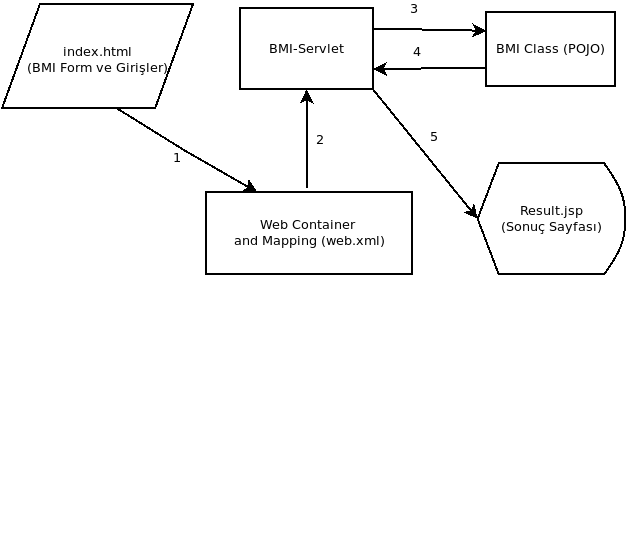
\includegraphics[scale=0.5]{/java/servlet}
\caption{Proje (webapp1) Akış Diagramı}
\label{fig:servletAkis}
\end{figure}
\lstinputlisting[label={list:bmi_index},caption={Index Sayfa Kodu},language={HTML},breaklines]{/home/cagatay/gitrepo/Ipa-ITBook/konular/java/projects/webProjects/webapp1/src/main/webapp/index.html}

Giriş sayfasından (Şekil \ref{fig:giris}) gelen request objesini servletimiz içerisine yazdığımız kodlarla parse edebiliyoruz. Mesela Liste (\ref{list:servlet}) de 11. satırda name parametresini request objesinden çekip program içerisinde string olarak tanımladığımız yine name isimli bir değişkene atıyoruz. Aynı şekilde giriş (index) sayfasından request objesine yazılan diğer parametreleri de çekiyoruz. Burade dikkatinizi celb edecek bir şey belki double tipinde olan değişkenleri, mesela kilo, double olarak almak için Double wrap classının parsırını kullanmamız ki bu parser string den double a değişkeni dönüştürmemizi sağlıyor. Zira request objesinin içindeki ifadeler string veya char biçiminde. Bunları direkt atamak hataya sebep olacaktır.  
\begin{figure}
	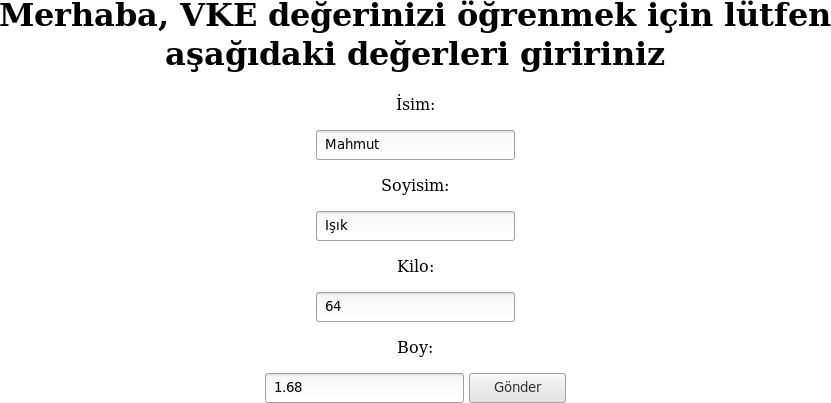
\includegraphics[scale=0.5]{/java/giris}
\centering\caption{Giriş (intex.html) Sayfası Görüntüsü}
	\label{fig:giris}
\end{figure}

\lstinputlisting[label={list:servlet},caption={Servlet Kodu},language={Java},breaklines]{/home/cagatay/gitrepo/Ipa-ITBook/konular/java/projects/webProjects/webapp1/src/main/java/com/stargate/BmiServlet.java}
Çekilen parametreleri daha sonra Liste (\ref{list:bmi.java}) de görülen Java classına hesap için gönderiyoruz. 

\lstinputlisting[label={list:bmi.java},caption={BMI Java Kodu},language={Java},breaklines]{/home/cagatay/gitrepo/Ipa-ITBook/konular/java/projects/webProjects/webapp1/src/main/java/com/stargate/BMI.java}

Liste \ref{list:servlet} da, 17. satırda BMI dan alınan sonucu result stringine depoluyoruz, daha sonra bu result ı 19. satırda bir attribute olarak request objesine ekliyoruz. 18, 20 ve 21 no` lu satırlar debug için koyduğumuz shell ekranına verileri basan satırlar. 22 nolu satırda request objesini view kısmına yani result.jsp sayfamıza aktarmak için view objesi tanımlıyoruz. 23 nolu satırda ise bu objenin forward methodu ile eklemeler yaptığımız request ve response objelerini sayfaya aktarıyoruz.
\lstinputlisting[label={list:result},caption={Sonuç Sayfa Kodu},breaklines]{/home/cagatay/gitrepo/Ipa-ITBook/konular/java/projects/webProjects/webapp1/src/main/webapp/WEB-INF/result.jsp}
Sonuç sayfasında ise yine request objesinden attributeları çekerek ekrana yazdırıyor ve view kısmını tamamlıyoruz.
\subsubsection{Mapping}

Şimdi gelelim mapping kısmına. Giriş sayfası  kodundan da (Liste \ref{list:bmi_index}) anlaşılacağı üzere formun action değeri satır 11 de  "bmi" olarak yazılmış, yani statik olarak düşünecek olursak form gönderildiğinde otomatik olarak açılacak (çalıştırılacak) sayfa/betik ismi "bmi". Oysa bizim bmi isimli bir sayfamız/betiğimiz/classımız yok ve formu işleyecek java classımızın ismi aslında "BMiServlet". İşte mapping olayı burada devreye giriyor. İster güvenlik gerekçesi, ister organizasyon kaygısı ile yapılsın, url mapping web geliştiriciliğin zor olmayan ama önemli bir parçasıdır. Standart bir projede mapping WEB-INF klasörü altında bulunan "web.xml" dosyası aracılığı ile yapılır. 
\lstinputlisting[label={list:webxml},caption={web.xml Mapping Dosyası İçeriği},language={XML},breaklines]{/home/cagatay/gitrepo/Ipa-ITBook/konular/java/projects/webProjects/webapp1/src/main/webapp/WEB-INF/web.xml}
web.xml içinde üç kademede servlet mapping yapıyoruz. Önce servlet name ile servletimize bir mahlas tanımlıyoruz, (mahlas "bmi" olmak zoruda değil aslında ama örneğimizde öyle tanımladık) bu mahlas için servlet class tanımlıyoruz ki bu class bizim BmiServletimiz. Daha sonra mapping kısmında bu mahlası bir url ile, index.html form action içinde referans verdiğimiz "bmi" ile ilişkilendiriyoruz. Artık herhangi bir sayfada /bmi url si çağırıldığında request objesi bizim servletimize gelecektir. 



